\clearpage
\twocolumn[{%
\rqparent
\subsection{Evaluation format}
\label{app:rq11_evaluation_recipe}

\noindent\begin{minipage}[t]{0.485\textwidth}
\vspace{0pt}
\paragraph{Research Question.} \emph{The rest of the analysis asks whether a cheap measurement reproduces the design decision of the 1.7B reference. This analysis turns that question into advice for a reader who has to choose what to evaluate. A \textbf{variant} of a benchmark is its items as published, their \texttt{rf\_} cloze rewrite (RF) or their \texttt{rfgm\_} LLM rewrite (LLM-RF), each scored by \textbf{accuracy} or by the gold answer's \textbf{bits per byte} (bBPB). For each benchmark, which variant recovers the reference's decision from the smallest proxy?}

\paragraph{Setup.} We compare the ways of evaluating a benchmark by the DA-size of the proxies 90M--1B against the 1.7B final checkpoint. We use the seed-1904 runs of every cell and every design pair, the multi-axis set, which also holds the single-axis pairs. This is the pair set of the surrogate comparison in the main text. On the single-axis pairs alone the best mean DA-size is 0.585 (LLM-RF bBPB at 90M), and LLM-RF bBPB $\rightarrow$ 1.7B bBPB falls to 0.65 at 600M, below 0.75. Each benchmark is read in up to six ways: its items as published, as RF or as LLM-RF, each scored by accuracy or by the bits per byte of the gold answer (bBPB). An accuracy variant counts on the tasks above chance at the proxy and at the reference. A bBPB variant has no chance level and is read against its original's 1.7B accuracy, so it counts where that accuracy is above chance.
\end{minipage}\hfill
\begin{minipage}[t]{0.485\textwidth}
\vspace{0pt}
\begin{rqfinding}
\textbf{1. No way of evaluating a benchmark reaches a mean DA-size of $\tau$ = 0.75 against the reference's accuracy decision at any proxy up to 1B.} The best mean is 0.63 (LLM-RF bBPB at 90M). Only the easier target, bBPB $\rightarrow$ 1.7B bBPB, clears $\tau$ (LLM-RF at 0.76--0.88 on 35 tasks). Against the same truth, bBPB beats the original accuracy at all five proxies (0.57--0.60 against 0.53--0.57 over every task, and 0.59--0.64 against 0.54--0.58 on the paired tasks). The rewrites help only when scored by bBPB: RF and LLM-RF accuracy reach 0.48--0.56 across the five proxies, and their bBPB 0.57--0.63. The eight benchmarks with the highest DA-size are drawn per variant along size and training (Figure~\ref{fig:app_rq11_recipe_by_benchmark}). (Figure~\ref{fig:app_rq11_evaluation_recipe}.)
\\
\\
\textbf{2. Against the same truth (bBPB $\rightarrow$ 1.7B accuracy), bBPB is the pick for 20 of the 36 benchmarks with a value and accuracy for 16.} Half of the bBPB picks (10 of 20) are never reliable and nine win only on the DA-size tie-break, while 14 of the 16 accuracy picks are the only variant that competes.
\\
\\
\textbf{3. The pick compares like with like.} A bBPB task is ranked on the same five proxies as an accuracy task, so a twin that dips below $\tau$ at 600M ranks later.
\end{rqfinding}
\end{minipage}

\vspace{\baselineskip}
\noindent\begin{minipage}{\textwidth}
\centering
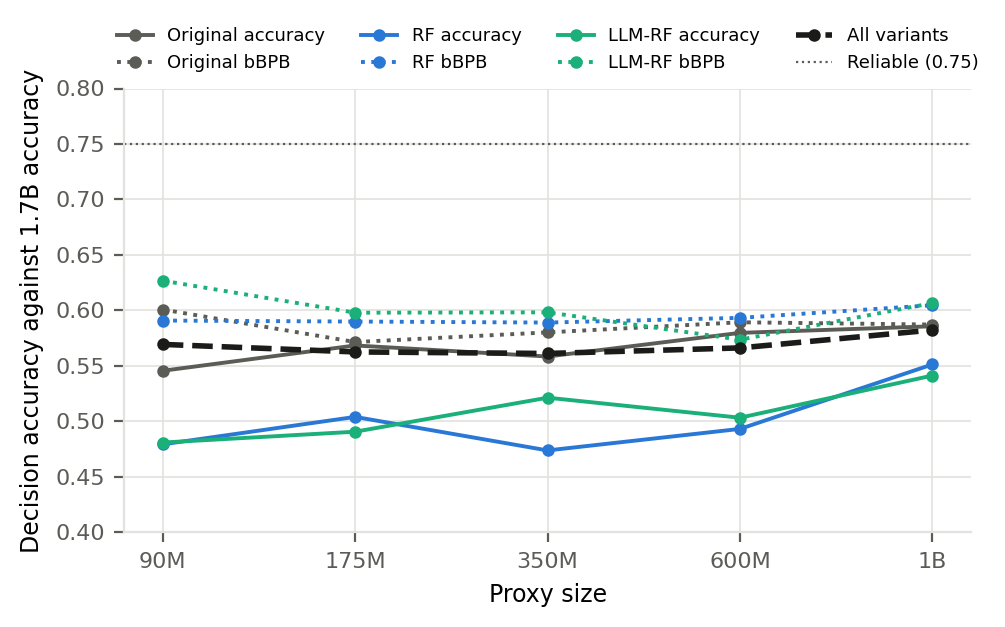
\includegraphics[width=\textwidth,height=0.36\textheight,keepaspectratio]{figures/app_rq11_evaluation_recipe.png}
% source: src/signal-and-noise/analysis/rq11_evaluation_recipe/pretraining/predictivity/recipe_da_size_variants_multi_axes_paper.png
\captionof{figure}{\textbf{No way of evaluating a benchmark reaches a mean DA-size of $\tau$ = 0.75 against the reference's accuracy decision at any proxy up to 1B.} Mean DA-size against the 1.7B accuracy for each way of reading a benchmark, by proxy size. The colour gives the item format (original, RF, LLM-RF) and the line style the score (solid for accuracy, dotted for bBPB). The dashed black line pools every variant and the dotted line marks 0.75.}
\label{fig:app_rq11_evaluation_recipe}
\end{minipage}
}]

\begin{figure*}[p]
\centering
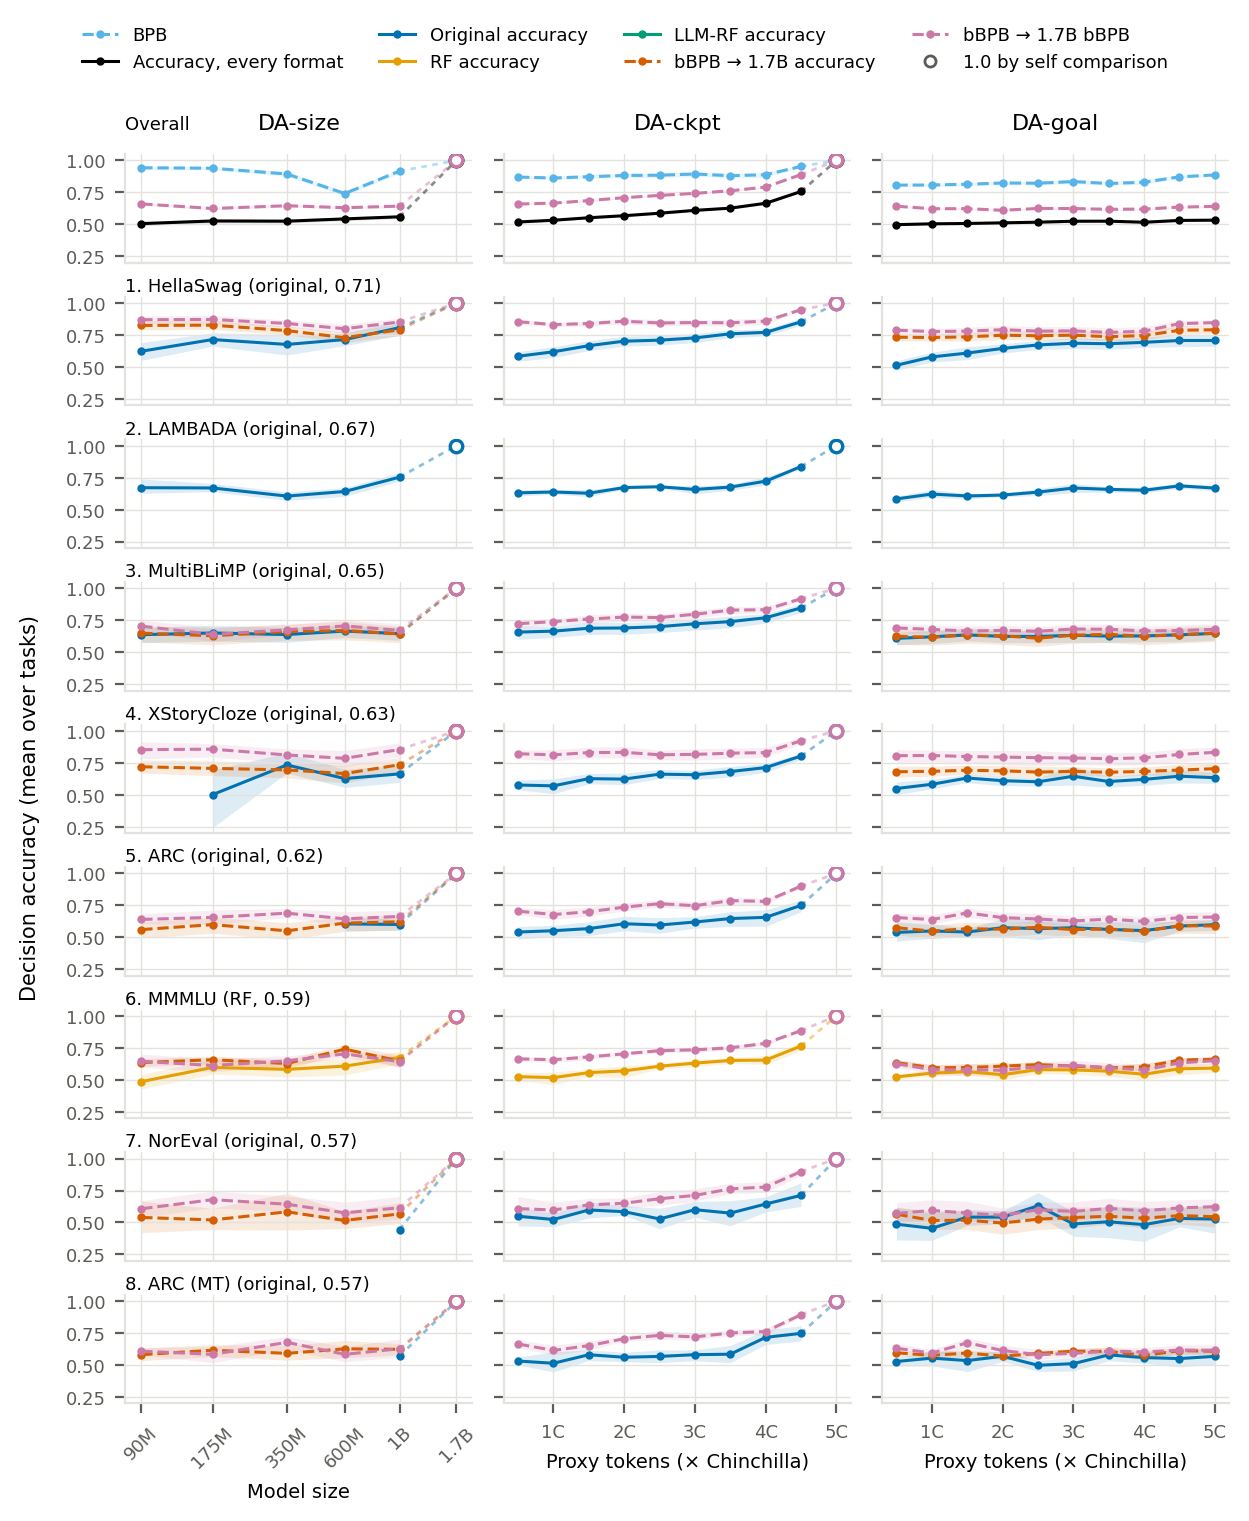
\includegraphics[width=\textwidth,height=0.8\textheight,keepaspectratio]{figures/app_rq11_recipe_by_benchmark.png}
% source: src/signal-and-noise/analysis/rq11_evaluation_recipe/pretraining/predictivity/recipe_da_all_by_benchmark_multi_axes_paper.png
\caption{\textbf{At the 90M proxy, a benchmark's bBPB read against the 1.7B accuracy ranks the design pairs more like the reference than its best accuracy format on 3 of the 3 top benchmarks where both have a value.} Overall, DA-size on accuracy goes from 0.51 at 90M to 0.56 at 1B, against 0.62--0.66 for the bBPB twins (read against the 1.7B bBPB) and 0.74--0.94 for BPB. The other rows are the 8 benchmarks with the highest mean DA-size over 90M--1B in their original or RF format (at least five tasks), ranked, with that format and value after the name. Columns: DA-size against the 1.7B final checkpoint, DA-ckpt against the proxy's own final checkpoint and DA-goal against the 1.7B final checkpoint, the last two averaged over the proxies 90M--1B. All use the multi-axis pairs of the seed-1904 runs, and accuracy is gated above chance. bBPB uses the twins of the ranking format, read against the 1.7B accuracy of the same items or against the 1.7B bBPB. The reading against accuracy has no DA-ckpt, because its reference would be a different score. LAMBADA has no twin. The bands are 95\% bootstrap intervals over tasks. A point on fewer than five tasks is not drawn. A hollow point is 1.0 because it compares a ranking with itself.}
\label{fig:app_rq11_recipe_by_benchmark}
\end{figure*}
